\begin{center}

  \begin{tabular}{rp{16cm}lp{20cm}}%{rl}

  % after \\: \hline or \cline{col1-col2} \cline{col3-col4} ...

  论文地址:& \href{https://dl.acm.org/doi/pdf/10.1145/2959100.2959190}{https://dl.acm.org/doi/pdf/10.1145/2959100.2959190} \\
  来源:& RecSys, 2016 \\
  作者:& Paul Covington, Jay Adams, Emre Sargin \\

  %源码:& \href{xxx}{xxx} \\

%  slides:& \href{http://yunshengb.com/wp-content/uploads/2017/03/nips_2018_r2l_workshop_talk.pdf}{{\footnotesize Convolutional Set Matching for Graph Similarity}}\\

  关键词:& \textbf{recommender system, deep learning, scalability} \\

  写于:& \date{2021-08-18}

  \end{tabular}

\end{center}

该论文\cite{covington2016deep}介绍了Youtube进行视频推荐的方法。Youtube进行视频推荐时分为两个阶段,各自由一个深度模型负责:deep candidate generation model、 deep ranking model。

\begin{figure}[h]
	\centering
	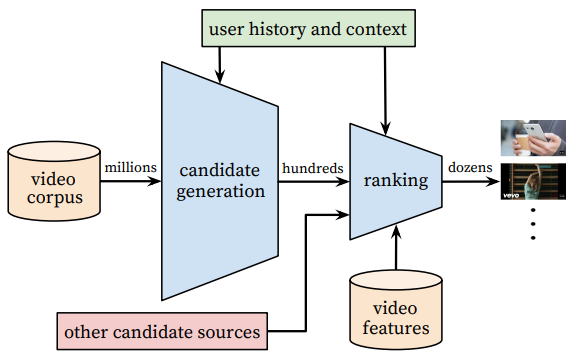
\includegraphics[width=.6\textwidth]{pics/recsys.png}
	\caption{推荐系统整体架构}
	\label{fig:recsys}
\end{figure}
\paragraph{问题定义}
在Youtube的视频推荐中主要有三大挑战:
\begin{itemize}
	\item Scale
	\item Fressness :每秒都有大量的视频上传到Youtube和大量用户产生观看记录,推荐的视频要能够反映最新上传的视频和用户最新的交互行为
	\item Noise :用户的历史行为是稀疏的且受到很多不可观测的因素的影响,一般难以得到用户的显示的对视频评价数据。需要在这样的数据上构建推荐算法
\end{itemize}
推荐系统的整体架构如Fig.\ref{fig:recsys}所示。


\paragraph{CANDIDATE GENERATION}
这一部分完成相关视频召回,召回阶段要保证高的Precision(尽量把相关的挑出来)。文中将召回作为一个多分类任务:
$$
P\left(w_{t}=i \mid U, C\right)=\frac{e^{v_{i} u}}{\sum_{j \in V} e^{v_{j} u}}
$$
$w_t$表示在时刻$t$看的视频的类别,每个视频$i$就是一个类别(没错,这是一个类别多达百万的多分类任务),$V, U, C$分别表示视频集、用户、上下文,$u \in \mathbb{R}^n, v_i \in \mathbb{R}^n$分别表示<用户,上下文>的向量、视频的向量。这一步模型的结构如Fig.\ref{fig:can_gen}所示,在最后一层输出的是\textit{user vector u},这个模型的目标是:\tbc{red}{学习一个函数,该函数以用户历史行为和上下文为输入,输出用户的embedding}

\begin{figure}[h]
	\centering
	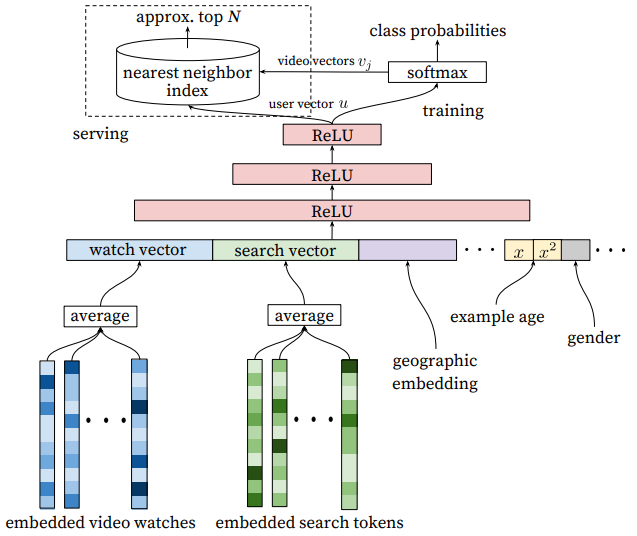
\includegraphics[width=.8\textwidth]{pics/candidate generation.png}
	\caption{Deep candidate generation model architecture}
	\label{fig:can_gen}
\end{figure}
嗯?不是说好的多分类吗,怎么变成了用户embedding了?在Fig.\ref{fig:can_gen}的顶部,最后一层的$Relu$的输出分别给到了serving和training两部分。送往training的部分确实会根据用户embedding计算类别概率,但是在serving时,是召回top N个视频,这时候只需要把用户embedding作为query在视频集里找到top N个相似的视频即可。

\subparagraph{训练数据的生成}为每个用户生成相同数量的训练样本,避免过于活跃的用户对损失函数产生过大的影响。而且由于涉及到极多类别的多分类问题,因此涉及到softmax的计算,为了加快速度,采用了负采样。

\subparagraph{特殊的特征}每秒都有大量的视频上传到Youtube,推荐最新上传的视频给用户是很重要的。一个视频在Youtube上的热门程度是不平稳的,但是召回模型对一个视频的预测的概率(热门程度)是平稳的,为了矫正这个问题,增加了一个$example age$特征,在训练时,样本的$example age$特征取值为$t_{max} - t_N$,其中$t_{max}$表示训练样本中最大的视频上传时间,$t_N$是样本的上传时间;在serving时,该特征为0.

\paragraph{RANKING}
这一部分对召回的视频进行排序,排序的依据是视频的期望观看时长,排序时要尽量保证高的Recall。如Fig.\ref{fig:ranking}所示,Ranking模型通过$weighted\:logistic$(\tbc{red}{在weighted LR中,输出样本$i$的odds会变成原来的$w_i$倍,$w_i$为$i$的权重})进行训练。

Ranking阶段的weighted LR中将正样本的观看时长作为样本权重,负样本的权重为1。通过训练得到了weighted LR的参数,得到每个视频被点击的概率,由于权重是视频时长,则odds就是该视频期望播放时长。

\begin{figure}[h]
	\centering
	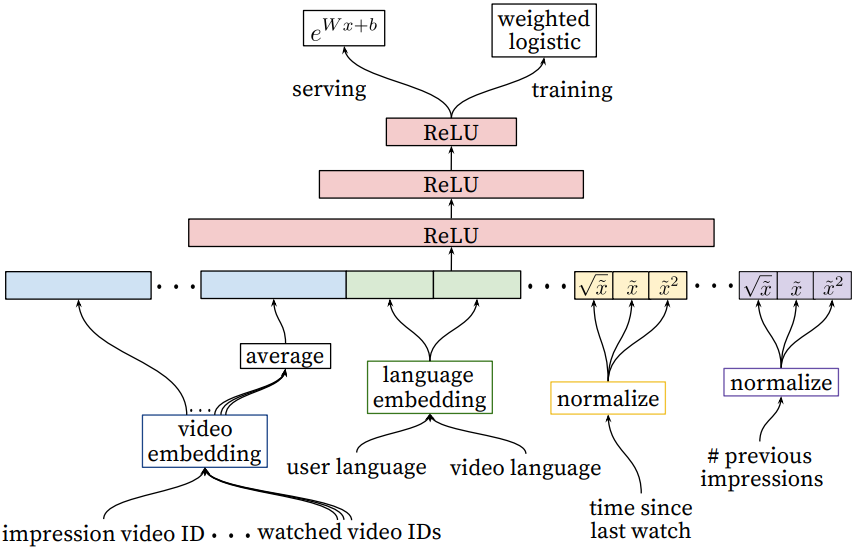
\includegraphics[width=.8\textwidth]{pics/ranking.png}
	\caption{Deep ranking network architecture}
	\label{fig:ranking}
\end{figure}

\subparagraph{特征表示}处理特征时忽略了时序,这样或许有助于模型的泛化。为一个视频打分时,该用户与这个视频(或相似视频)之前的交互数据最具参考价值。

\paragraph{总结}

\begin{itemize}
	\item 将召回阶段作为一个极多类别的分类任务
	\item 排序阶段预测每个视频的期望播放时长
	\item 特征工程功不可没
\end{itemize}

